\documentclass[crop,tikz]{standalone}

\tikzset{>=latex}
\usetikzlibrary{decorations.markings,calc}
\colorlet{green}{black!40!green}

\begin{document}
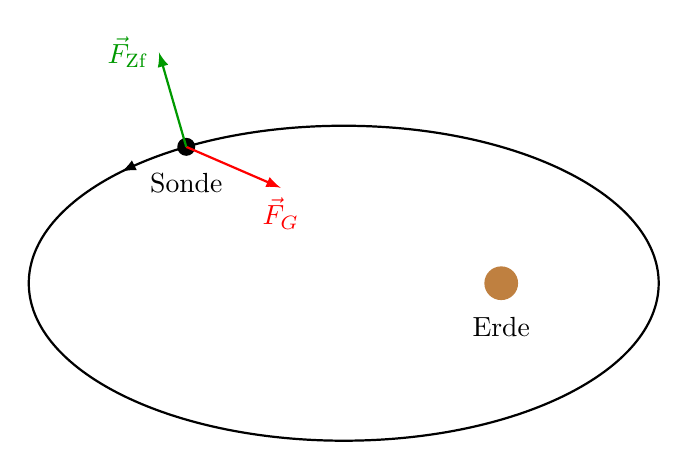
\begin{tikzpicture}[scale=2,thick]
  \pgfmathsetmacro{\ra}{2}
  \pgfmathsetmacro{\rb}{1}
  \coordinate (C) at (0,0); % center of ellipse
  \coordinate (E) at (1,0); % Earth
  \coordinate (S) at (-1,{\rb*sqrt(1 - (-1)^2/\ra^2)}); % Satellite
  % Ellipse
  \draw[decoration={markings, mark=at position 0.4 with {\arrow{>}}},
        postaction={decorate}] (C) ellipse ({\ra} and {\rb});
  % Earth
  \draw[fill,brown] (E) circle (0.1) node[below=0.3cm,black] {Erde};
  % Sattelite
  \draw[fill] (S) circle (0.05) node[below=0.2cm,black] {Sonde};
  % Gravity
  \coordinate (FG) at ($(S)!0.3!(E)$);
  \draw[->,red] (S) -- (FG) node[below] {$\vec{F}_G$};
  % incorrect centrifugal force
  \coordinate (FZ) at ($(S)+0.6*({\rb*((-1)/\ra^2)/sqrt(1 - (-1)^2/\ra^2)},1)$);
  \draw[->,green] (S) -- (FZ) node[left] {$\vec{F}_{\rm Zf}$};
\end{tikzpicture}
\end{document}
